% ============================================================
% FEE3411 Control Systems A -- Tutorial sheet, Week 01
% Topic: Mathematical toolkit review
%
% ONE source, TWO outputs. The solutions toggle is driven by \jobname,
% so the two PDFs cannot drift apart:
%
%   latexmk -pdf -jobname=week-01-tutorial-questions week-01-tutorial.tex
%   latexmk -pdf -jobname=week-01-tutorial-solutions week-01-tutorial.tex
%
% Needs: ../tex/preamble.tex (this file lives in Tutorials/).
% ============================================================
\documentclass[11pt,a4paper]{article}
\usepackage[margin=25mm]{geometry}
% ============================================================
% FEE3411 Control Systems A -- shared preamble
% Used by both the lecture notes (article) and the slides (beamer).
% ============================================================
\usepackage[T1]{fontenc}
% lmodern gives cleaner PDF fonts but is absent from minimal TeX installs.
% Load it only if present, so this preamble builds anywhere.
\IfFileExists{lmodern.sty}{\usepackage{lmodern}}{}
\usepackage{amsmath,amssymb,amsthm}
\usepackage{graphicx}
\usepackage{booktabs}
\usepackage{siunitx}
\usepackage{tikz}
\usepackage{circuitikz}
\usepackage{pgfplots}
\pgfplotsset{compat=1.18}
\usetikzlibrary{arrows.meta,positioning,calc,decorations.markings,shapes.geometric}
\usepackage[most]{tcolorbox}
\usepackage{xcolor}

% ---- Course colours -------------------------------------------------
\definecolor{fnavy}{HTML}{1F3864}
\definecolor{faccent}{HTML}{2E5E4E}
\definecolor{fflag}{HTML}{9C4221}

% ---- Block-diagram style --------------------------------------------
\tikzset{
  block/.style   = {draw, thick, rectangle, minimum height=2.6em,
                    minimum width=3.2em, align=center},
  sumnode/.style = {draw, thick, circle, inner sep=0pt, minimum size=1.6em},
  pickoff/.style = {fill, circle, inner sep=0pt, minimum size=3pt},
  sig/.style     = {-{Latex[length=2mm]}, thick},
}

% ---- Summing-junction signs -----------------------------------------
% \sumsign{<node>}{<angle>}{<+ or ->} places a sign just outside the circle.
\newcommand{\sumsign}[3]{\node[font=\small] at ($(#1)+(#2:0.5)$) {$#3$};}

% ---- Boxed environments ---------------------------------------------
\newtcolorbox{keyidea}[1][]{colback=fnavy!5,colframe=fnavy,
  fonttitle=\bfseries,title=Key idea,#1}
\newtcolorbox{workedex}[1][]{colback=faccent!5,colframe=faccent,
  fonttitle=\bfseries,title=Worked example,#1}
\newtcolorbox{pitfall}[1][]{colback=fflag!5,colframe=fflag,
  fonttitle=\bfseries,title=Common pitfall,#1}

% ---- Shorthands ------------------------------------------------------
\newcommand{\Lap}{\mathcal{L}}
\newcommand{\jw}{\mathrm{j}\omega}
\newcommand{\wn}{\omega_{n}}
\newcommand{\zt}{\zeta}
\newcommand{\TF}[1]{#1(s)}

% ---- Week title machinery -------------------------------------------
\usepackage{fancyhdr}
\newcommand{\thecoursecode}{FEE3411}
\newcommand{\thecoursename}{Control Systems A}
\newcommand{\wknum}{}
\newcommand{\wktopic}{}
\newcommand{\weeknumber}[1]{\renewcommand{\wknum}{#1}}
\newcommand{\weektopic}[1]{\renewcommand{\wktopic}{#1}}
\newcommand{\weektitle}{%
  \thispagestyle{plain}%
  \begin{center}
    {\large\sffamily\bfseries\color{fnavy}\thecoursecode: \thecoursename}\\[2pt]
    {\Huge\sffamily\bfseries Week \wknum}\\[4pt]
    {\LARGE\sffamily\color{fnavy}\wktopic}\\[6pt]
    \rule{\textwidth}{1.2pt}
  \end{center}\vspace{4pt}%
  \pagestyle{fancy}\fancyhf{}%
  \fancyhead[L]{\footnotesize\color{gray}\thecoursecode\ Week \wknum\ --- \wktopic}%
  \fancyhead[R]{\footnotesize\color{gray}\thepage}%
  \renewcommand{\headrulewidth}{0.4pt}%
}

% ---- Outcomes and reading boxes -------------------------------------
\newenvironment{outcomes}
  {\begin{tcolorbox}[colback=white,colframe=fnavy!60,
      fonttitle=\bfseries,title=By the end of this week you should be able to]
   \begin{itemize}[leftmargin=*]}
  {\end{itemize}\end{tcolorbox}}

\newtcolorbox{readingbox}{colback=gray!5,colframe=gray!50,
  fonttitle=\bfseries,title=Reading}

% enumitem must NOT be loaded under beamer: it overwrites beamer's itemize
% templates and the bullet markers silently disappear. The notes (article) get
% it; the slides (beamer) use beamer's own list machinery instead.
\makeatletter
\@ifclassloaded{beamer}{}{\usepackage{enumitem}}
\makeatother

\usepackage{environ}

% ---- solutions toggle, decided by the job name ----------------------
% NB: xstring's \IfSubStr does NOT work here -- \jobname yields catcode-12
% characters and the comparison silently fails, giving the questions version
% both times. The expl3 string test below is catcode-blind and does work.
\newif\ifsolutions
\ExplSyntaxOn
\tl_set:Nx \l_tmpa_tl { \jobname }
\str_if_in:NnTF \l_tmpa_tl { solutions } { \solutionstrue } { \solutionsfalse }
\ExplSyntaxOff

\newtcolorbox{solbox}[1][]{colback=faccent!4,colframe=faccent!70,
  fonttitle=\bfseries,title=Solution,breakable,#1}
\NewEnviron{solution}{\ifsolutions\begin{solbox}\BODY\end{solbox}\fi}

% ---- question tagging ------------------------------------------------
\newcommand{\inhour}{\hfill{\small\color{faccent}\itshape[in the hour]}}
\newcommand{\athome}{\hfill{\small\color{fflag}\itshape[homework]}}

\weeknumber{1}
\weektopic{Tutorial 1 --- Mathematical Toolkit Review}

\begin{document}
\weektitle

\begin{center}
\ifsolutions
  {\large\sffamily\bfseries\color{fflag}QUESTIONS AND SOLUTIONS}\\[2pt]
  {\small\itshape Instructor copy --- do not circulate before the tutorial.}
\else
  {\large\sffamily\bfseries\color{fnavy}QUESTION SHEET}
\fi
\end{center}

\bigskip
\noindent
This hour is a \textbf{review}, not new material. Everything here you have met
in FEE~222 or FEE~372; the purpose is to get it back into working order,
because from Week~2 onwards it is assumed silently in every derivation.

\smallskip
\noindent
Questions marked \textbf{\color{faccent}[in the hour]} are the ones we work
through together. Those marked \textbf{\color{fflag}[homework]} you do in your
own time --- they are not collected, but Week~2 assumes you have done them.

\smallskip
\noindent
\emph{Preparation:} Khalil Appendix~A (p.~438) or Nise \S2.2 (p.~35).

% --------------------------------------------------------------------
\begin{readingbox}
\textbf{The toolkit you should be able to use without looking anything up.}

\smallskip
\begin{minipage}[t]{0.35\textwidth}
\textbf{Pairs}\\[2pt]
\footnotesize
\begin{tabular}{@{}ll@{}}
$\delta(t)$ & $1$\\
$u(t)$ & $1/s$\\
$t$ & $1/s^{2}$\\
$t^{n}/n!$ & $1/s^{n+1}$\\
$e^{-at}$ & $1/(s+a)$\\
$t e^{-at}$ & $1/(s+a)^{2}$\\
$\sin\omega t$ & $\omega/(s^{2}+\omega^{2})$\\
$\cos\omega t$ & $s/(s^{2}+\omega^{2})$\\
$e^{-at}\sin\omega t$ & $\omega/[(s+a)^{2}+\omega^{2}]$\\
$e^{-at}\cos\omega t$ & $(s+a)/[(s+a)^{2}+\omega^{2}]$\\
\end{tabular}
\end{minipage}
\hfill
\begin{minipage}[t]{0.58\textwidth}
\textbf{Properties}\\[2pt]
\footnotesize
\begin{tabular}{@{}ll@{}}
Linearity & $\Lap\{af+bg\}=aF+bG$\\
Differentiation & $\Lap\{\dot f\}=sF(s)-f(0^{-})$\\
 & $\Lap\{\ddot f\}=s^{2}F(s)-s f(0^{-})-\dot f(0^{-})$\\
Integration & $\Lap\left\{\int_{0}^{t}\!f\right\}=F(s)/s$\\
Frequency shift & $\Lap\{e^{-at}f(t)\}=F(s+a)$\\
Time shift & $\Lap\{f(t-T)u(t-T)\}=e^{-sT}F(s)$\\
Initial value & $f(0^{+})=\lim_{s\to\infty}sF(s)$\\
Final value & $f(\infty)=\lim_{s\to 0}sF(s)$\\
 & \emph{only if all poles of $sF(s)$}\\
 & \emph{have negative real parts}\\
\end{tabular}
\end{minipage}
\end{readingbox}

% ====================================================================
\section*{Question 1 --- Standard test signals \inhour}

\begin{enumerate}[label=(\alph*)]
\item Sketch, on the same time axis, the unit impulse $\delta(t)$, unit step
      $u(t)$, unit ramp $r(t)=t\,u(t)$ and unit parabola
      $p(t)=\tfrac{1}{2}t^{2}u(t)$. Write down the Laplace transform of each.

\item Show that each signal in the list is the time integral of the one before
      it. Using the integration property only, deduce the transforms
      $1/s$, $1/s^{2}$, $1/s^{3}$ from $\Lap\{\delta\}=1$.

\item Why does a control engineer test with \emph{these} signals rather than,
      say, a sine wave or a recorded real input?
\end{enumerate}

\begin{solution}
\textbf{(a)} $\Lap\{\delta\}=1$, $\Lap\{u\}=1/s$, $\Lap\{r\}=1/s^{2}$,
$\Lap\{p\}=1/s^{3}$. The sketches: an arrow of unit area at the origin; a step
to 1; a straight line of unit slope; an upward parabola.

\medskip
\textbf{(b)} $u(t)=\int_{0}^{t}\delta(\tau)\,d\tau$,
$r(t)=\int_{0}^{t}u(\tau)\,d\tau$, $p(t)=\int_{0}^{t}r(\tau)\,d\tau$. Each
integration divides the transform by $s$, so
$1\to 1/s\to 1/s^{2}\to 1/s^{3}$.

\medskip
\textbf{(c)} Three reasons.
\begin{itemize}
\item They form a \emph{ladder of difficulty}: a step asks the system to reach
      a new constant value, a ramp to follow a constant velocity, a parabola a
      constant acceleration. In Week~6 we will see that a given system tracks
      some of these with zero error, some with finite error, and some not at
      all --- that classification is \emph{system type}.
\item They are simple enough that the response can be worked out by hand, so
      the answer is a formula you can reason about, not a number from a
      simulation.
\item Any realistic input can be built from them (or from impulses), so if you
      know the response to these you know a great deal about the response to
      everything else.
\end{itemize}
\emph{Sine waves are not neglected} --- the entire frequency-response half of
this unit, Weeks 9--12, is the sinusoidal steady-state response.
\end{solution}

% ====================================================================
\section*{Question 2 --- Transforms and properties \inhour}

\begin{enumerate}[label=(\alph*)]
\item From the definition $F(s)=\int_{0^{-}}^{\infty}f(t)e^{-st}\,dt$, derive
      $\Lap\{e^{-at}\}$. For which values of $s$ does the integral converge?

\item Using the properties in the box, and \emph{without} integrating, find
      \[
        \text{(i) } \Lap\{t\,e^{-3t}\}\qquad
        \text{(ii) } \Lap\{e^{-2t}\sin 4t\}\qquad
        \text{(iii) } \Lap\{e^{-(t-2)}u(t-2)\}
      \]

\item Find $F(s)$ for $f(t)=5-3e^{-2t}\cos 4t$.

\item For $\displaystyle F(s)=\frac{10(s+2)}{s(s^{2}+4s+13)}$, find
      $f(0^{+})$ and $f(\infty)$ without inverting.

\item A student applies the final value theorem to
      $\displaystyle G(s)=\frac{5}{s^{2}+9}$ and reports $g(\infty)=0$.
      What has gone wrong?
\end{enumerate}

\begin{solution}
\textbf{(a)}
\[
  \Lap\{e^{-at}\}=\int_{0}^{\infty}e^{-at}e^{-st}dt
  =\int_{0}^{\infty}e^{-(s+a)t}dt
  =\left[\frac{-e^{-(s+a)t}}{s+a}\right]_{0}^{\infty}
  =\frac{1}{s+a}.
\]
The upper limit vanishes only if $\mathrm{Re}(s+a)>0$, i.e.\
$\mathrm{Re}(s)>-a$. That half-plane is the \emph{region of convergence}. We
almost never mention it again, because in this unit the transform is a
bookkeeping device rather than an object of study --- but it is the reason the
pole sits at $s=-a$.

\medskip
\textbf{(b)}
\begin{enumerate}[label=(\roman*)]
\item Frequency shift applied to $\Lap\{t\}=1/s^{2}$:
      $\;\Lap\{t e^{-3t}\}=\dfrac{1}{(s+3)^{2}}$.
\item Frequency shift applied to $\Lap\{\sin 4t\}=4/(s^{2}+16)$:
      $\;\dfrac{4}{(s+2)^{2}+16}$.
\item Time shift with $T=2$ applied to $\Lap\{e^{-t}\}=1/(s+1)$:
      $\;\dfrac{e^{-2s}}{s+1}$.
\end{enumerate}

\begin{pitfall}
In (iii) the exponent is $-(t-2)$, \emph{not} $-t$, and the step is
$u(t-2)$. Both must be shifted by the same amount or the time-shift property
does not apply. $\Lap\{e^{-t}u(t-2)\}$ is a different (and messier) problem:
write $e^{-t}=e^{-2}e^{-(t-2)}$ first, giving $e^{-2}e^{-2s}/(s+1)$.
\end{pitfall}

\medskip
\textbf{(c)} $\Lap\{5\}=5/s$ and, by frequency shift,
$\Lap\{e^{-2t}\cos 4t\}=(s+2)/[(s+2)^{2}+16]$. Hence
\[
  F(s)=\frac{5}{s}-\frac{3(s+2)}{(s+2)^{2}+16}
      =\frac{5}{s}-\frac{3(s+2)}{s^{2}+4s+20}
      =\frac{2(s^{2}+7s+50)}{s(s^{2}+4s+20)} .
\]

\medskip
\textbf{(d)} Initial value:
\[
  f(0^{+})=\lim_{s\to\infty}sF(s)
   =\lim_{s\to\infty}\frac{10s(s+2)}{s^{2}+4s+13}=10 .
\]
Final value: the poles of $sF(s)$ are the roots of $s^{2}+4s+13$, namely
$s=-2\pm j3$, both with negative real part, so the theorem applies:
\[
  f(\infty)=\lim_{s\to 0}sF(s)=\frac{10\times 2}{13}=\frac{20}{13}\approx 1.538 .
\]

\medskip
\textbf{(e)} The theorem has been applied where it is not valid. The poles of
$sG(s)=5s/(s^{2}+9)$ are at $s=\pm j3$ --- on the imaginary axis, not strictly
in the left half-plane. In fact $g(t)=\tfrac{5}{3}\sin 3t$, which oscillates
forever and has no final value at all.

\begin{pitfall}
The final value theorem returns a number whether or not it is entitled to.
\textbf{Always check the poles of $sF(s)$ first.} This trap reappears in Week~6
whenever a steady-state error is computed for a system that is not actually
stable --- the algebra produces a tidy answer for a system that is in fact
running away.
\end{pitfall}
\end{solution}

% ====================================================================
\section*{Question 3 --- Partial fractions \inhour}

Expand each of the following and hence find $f(t)$. In each case check your
answer against the initial and final value theorems.

\begin{enumerate}[label=(\alph*)]
\item $\displaystyle F(s)=\frac{s+3}{s(s+1)(s+2)}$ \hfill (distinct real poles)
\item $\displaystyle F(s)=\frac{s+4}{s(s+2)^{2}}$ \hfill (a repeated pole)
\item $\displaystyle F(s)=\frac{10}{s(s^{2}+2s+5)}$ \hfill (a complex pair)
\end{enumerate}

For (c), also read off the undamped natural frequency $\wn$ and damping ratio
$\zt$ of the quadratic factor.

\begin{solution}
\textbf{(a)} Write $F=\dfrac{A}{s}+\dfrac{B}{s+1}+\dfrac{C}{s+2}$ and use the
cover-up rule:
\[
  A=\left.\frac{s+3}{(s+1)(s+2)}\right|_{s=0}=\frac{3}{2},\quad
  B=\left.\frac{s+3}{s(s+2)}\right|_{s=-1}=\frac{2}{(-1)(1)}=-2,
\]
\[
  C=\left.\frac{s+3}{s(s+1)}\right|_{s=-2}=\frac{1}{(-2)(-1)}=\frac{1}{2}.
\]
\[
  \boxed{\;f(t)=\tfrac{3}{2}-2e^{-t}+\tfrac{1}{2}e^{-2t}\;}
\]
\emph{Checks.} $f(0)=1.5-2+0.5=0$, and indeed $sF(s)\to 0$ as $s\to\infty$
($F$ is strictly proper by two degrees). $f(\infty)=1.5$, matching
$\lim_{s\to 0}sF(s)=3/2$.

\medskip
\textbf{(b)} With a repeated pole the expansion is
$F=\dfrac{A}{s}+\dfrac{B}{s+2}+\dfrac{C}{(s+2)^{2}}$.
\[
  A=\left.\frac{s+4}{(s+2)^{2}}\right|_{s=0}=\frac{4}{4}=1,
  \qquad
  C=\left.\frac{s+4}{s}\right|_{s=-2}=\frac{2}{-2}=-1 .
\]
For $B$, multiply through by $(s+2)^{2}$ and differentiate before substituting:
\[
  B=\left.\frac{d}{ds}\!\left[\frac{s+4}{s}\right]\right|_{s=-2}
   =\left.\frac{d}{ds}\!\left[1+\frac{4}{s}\right]\right|_{s=-2}
   =\left.-\frac{4}{s^{2}}\right|_{s=-2}=-1 .
\]
\[
  F(s)=\frac{1}{s}-\frac{1}{s+2}-\frac{1}{(s+2)^{2}}
  \qquad\Longrightarrow\qquad
  \boxed{\;f(t)=1-e^{-2t}-t\,e^{-2t}\;}
\]
\emph{Checks.} $f(0)=1-1-0=0$; $f(\infty)=1=\lim_{s\to0}sF(s)=4/4$.

\begin{pitfall}
The commonest error here is to forget the $B$ term entirely, or to try to find
it by the cover-up rule (which gives $\infty$). A pole of multiplicity $m$
contributes $m$ terms, and all but the highest need the derivative trick.
\end{pitfall}

\medskip
\textbf{(c)} The quadratic $s^{2}+2s+5$ has roots $s=-1\pm j2$, which do not
factorise over the reals, so keep it whole:
\[
  F(s)=\frac{A}{s}+\frac{Bs+C}{s^{2}+2s+5},\qquad
  A=\left.\frac{10}{s^{2}+2s+5}\right|_{s=0}=2 .
\]
Multiplying up, $10=2(s^{2}+2s+5)+(Bs+C)s$, so matching coefficients gives
$B=-2$ and $C=-4$. Now complete the square, $s^{2}+2s+5=(s+1)^{2}+2^{2}$, and
split the numerator so that each piece matches a table entry:
\[
  \frac{2s+4}{(s+1)^{2}+2^{2}}
  =\frac{2(s+1)}{(s+1)^{2}+2^{2}}+\frac{2}{(s+1)^{2}+2^{2}} .
\]
Hence
\[
  F(s)=\frac{2}{s}-\frac{2(s+1)}{(s+1)^{2}+2^{2}}-\frac{2}{(s+1)^{2}+2^{2}}
\]
\[
  \boxed{\;f(t)=2-2e^{-t}\cos 2t-e^{-t}\sin 2t\;}
\]
(the last term because $\Lap^{-1}\{2/[(s+1)^{2}+4]\}=e^{-t}\sin 2t$, the table
entry needing $\omega=2$ in the numerator).

\emph{Checks.} $f(0)=2-2-0=0$; $f(\infty)=2=\lim_{s\to0}sF(s)=10/5$.

\medskip
Comparing $s^{2}+2s+5$ with the standard form $s^{2}+2\zt\wn s+\wn^{2}$:
\[
  \wn=\sqrt{5}\approx\SI{2.236}{\radian\per\second},
  \qquad
  2\zt\wn=2 \;\Rightarrow\; \zt=\frac{1}{\sqrt{5}}\approx 0.447 .
\]
Since $0<\zt<1$ the response is \textbf{underdamped}, and the damped frequency
$\omega_{d}=\wn\sqrt{1-\zt^{2}}=2$ is exactly the $2$ appearing in
$\sin 2t$ and $\cos 2t$. Week~5 does nothing to this result except give the
quantities names.
\end{solution}

% ====================================================================
\section*{Question 4 --- Complex numbers and the $s$-plane \inhour}

This question is the one that pays off most later: the graphical evaluation in
part (b) is the whole basis of root-locus sketching in Week~8 and of Bode and
Nyquist plots in Weeks 10--12.

\medskip
Consider
\[
  G(s)=\frac{4(s+2)}{s(s+4)} .
\]

\begin{enumerate}[label=(\alph*)]
\item Mark the poles ($\times$) and zeros ($\circ$) of $G$ on an $s$-plane
      diagram.

\item Evaluate $G(s)$ at the point $s=-1+j$ \textbf{graphically}: draw the
      vector from each pole and zero to that point, measure (or compute) its
      length and angle, and combine them. Confirm your answer algebraically.

\item A second-order system has poles at $s=-1\pm j2$. Write down the form of
      the corresponding time-domain term. On a sketch of the $s$-plane, mark
      $\wn$ and the angle $\theta$ from the negative real axis, and show that
      $\zt=\cos\theta$. Evaluate both.

\item In one sentence each: what does the \emph{real} part of a pole control,
      and what does the \emph{imaginary} part control?
\end{enumerate}

\begin{solution}
\textbf{(a)} Zero at $s=-2$; poles at $s=0$ and $s=-4$.

\begin{center}
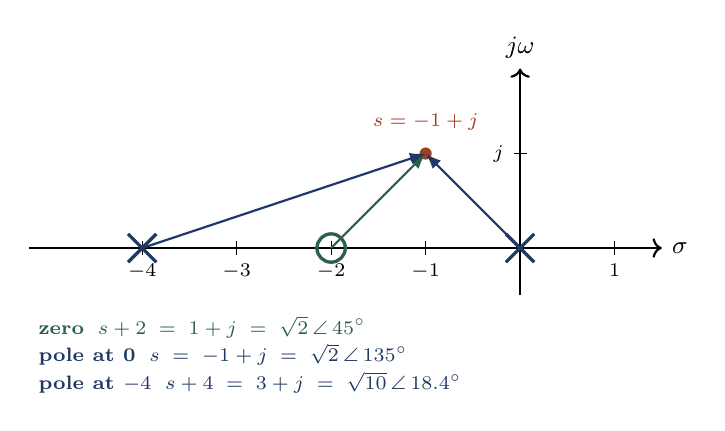
\begin{tikzpicture}[x=1.2cm, y=1.2cm, font=\small]
\draw[->,thick] (-5.2,0) -- (1.5,0) node[right] {$\sigma$};
\draw[->,thick] (0,-0.5) -- (0,1.9) node[above] {$j\omega$};
\foreach \x in {-4,-3,-2,-1,1}
  \draw (\x,0.07) -- (\x,-0.07) node[below,font=\scriptsize] {$\x$};
\draw (0.07,1) -- (-0.07,1) node[left,font=\scriptsize] {$j$};
% ---- poles (x) and zero (o) ----
\draw[very thick,fnavy] (-0.15,-0.15) -- (0.15,0.15);
\draw[very thick,fnavy] (-0.15,0.15) -- (0.15,-0.15);
\draw[very thick,fnavy] (-4.15,-0.15) -- (-3.85,0.15);
\draw[very thick,fnavy] (-4.15,0.15) -- (-3.85,-0.15);
\draw[very thick,faccent] (-2,0) circle (0.15);
% ---- test point ----
\fill[fflag] (-1,1) circle (2.2pt);
\node[fflag,anchor=south,font=\scriptsize] at (-1,1.14) {$s=-1+j$};
% ---- the three vectors ----
\draw[sig,faccent] (-2,0) -- (-1,1);
\draw[sig,fnavy]   (0,0)  -- (-1,1);
\draw[sig,fnavy]   (-4,0) -- (-1,1);
% ---- legend, clear of the diagram ----
\node[anchor=north west,font=\scriptsize,align=left] at (-5.2,-0.62)
  {\textcolor{faccent}{\textbf{zero} $\;s+2 \;=\; 1+j
      \;=\; \sqrt{2}\,\angle\,\ang{45}$}\\[2pt]
   \textcolor{fnavy}{\textbf{pole at 0} $\;s \;=\; -1+j
      \;=\; \sqrt{2}\,\angle\,\ang{135}$}\\[2pt]
   \textcolor{fnavy}{\textbf{pole at $-4$} $\;s+4 \;=\; 3+j
      \;=\; \sqrt{10}\,\angle\,\ang{18.4}$}};
\end{tikzpicture}
\end{center}

\textbf{(b)} At $s=-1+j$ each factor is a vector \emph{from} the critical point
\emph{to} the test point:
\[
\begin{array}{lll}
  s+2 = 1+j & |s+2|=\sqrt{2} & \angle(s+2)=\ang{45}\\
  s     = -1+j & |s|=\sqrt{2} & \angle s=\ang{135}\\
  s+4 = 3+j & |s+4|=\sqrt{10} & \angle(s+4)=\arctan\tfrac{1}{3}=\ang{18.435}
\end{array}
\]
Magnitudes of numerator factors divide by magnitudes of denominator factors;
angles subtract:
\[
  |G|=\frac{4\sqrt{2}}{\sqrt{2}\,\sqrt{10}}=\frac{4}{\sqrt{10}}=1.265,
  \qquad
  \angle G=\ang{45}-\ang{135}-\ang{18.435}=\ang{-108.435}.
\]
\emph{Algebraic check.}
\[
  G(-1+j)=\frac{4(1+j)}{(-1+j)(3+j)}=\frac{4+4j}{-4+2j}=-0.4-1.2j,
\]
whose magnitude is $\sqrt{0.16+1.44}=1.265$ and whose angle is
$\ang{-108.435}$. \checkmark

\begin{keyidea}
A transfer function evaluated at a point is nothing but \emph{a product of
vector lengths divided by another product of vector lengths, with the angles
subtracted}. Every graphical method in the second half of this unit ---
the root-locus angle and magnitude conditions, the shape of a Bode plot near a
corner, the shape of a Nyquist contour --- is this one fact applied at
different sets of points.
\end{keyidea}

\medskip
\textbf{(c)} Poles at $s=-1\pm j2$ correspond to the time-domain term
\[
  e^{-t}\left(A\cos 2t+B\sin 2t\right)
  \quad\text{equivalently}\quad
  Ce^{-t}\sin(2t+\phi).
\]
On the $s$-plane, $\wn$ is the \emph{distance from the origin} to the pole and
$\theta$ the angle it makes with the negative real axis:
\[
  \wn=\sqrt{1^{2}+2^{2}}=\sqrt{5}=2.236,
  \qquad
  \cos\theta=\frac{1}{\sqrt 5}=0.447
  \;\Rightarrow\; \theta=\ang{63.43}.
\]
Writing the pole as $-\zt\wn\pm j\wn\sqrt{1-\zt^{2}}$, the horizontal distance
is $\zt\wn$ and the hypotenuse is $\wn$, so
$\cos\theta=\zt\wn/\wn=\zt$. Hence $\zt=0.447$, the same value as in
Question 3(c) --- the same quadratic.

\begin{center}
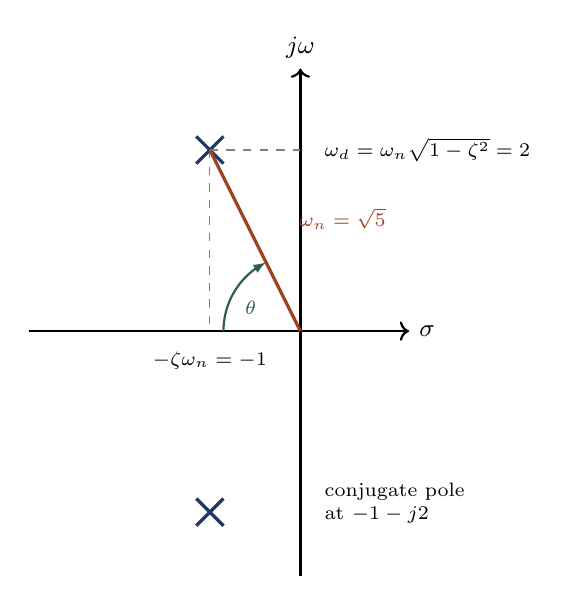
\begin{tikzpicture}[x=1.15cm, y=1.15cm, font=\small]
\draw[->,thick] (-3.0,0) -- (1.2,0) node[right] {$\sigma$};
\draw[->,thick] (0,-2.7) -- (0,2.9) node[above] {$j\omega$};
% ---- the conjugate pair ----
\foreach \y in {2,-2}{
  \draw[very thick,fnavy] (-1.15,{\y-0.15}) -- (-0.85,{\y+0.15});
  \draw[very thick,fnavy] (-1.15,{\y+0.15}) -- (-0.85,{\y-0.15});}
% ---- construction lines ----
\draw[dashed,gray] (-1,2) -- (-1,0);
\draw[dashed,gray] (-1,2) -- (0,2);
\draw[very thick,fflag] (0,0) -- (-1,2);
% ---- labels, all clear of the lines ----
\node[anchor=north,font=\scriptsize] at (-1,-0.12) {$-\zt\wn=-1$};
\node[anchor=west,font=\scriptsize] at (0.16,2.0) {$\omega_{d}=\wn\sqrt{1-\zt^{2}}=2$};
\node[fflag,anchor=west,font=\scriptsize] at (-0.12,1.24) {$\wn=\sqrt{5}$};
\draw[thick,-{Latex[length=1.6mm]},faccent] (-0.85,0) arc (180:116.57:0.85);
\node[faccent,font=\scriptsize] at (-0.55,0.26) {$\theta$};
\node[anchor=west,font=\scriptsize,align=left] at (0.16,-1.9)
     {conjugate pole\\ at $-1-j2$};
\end{tikzpicture}
\end{center}

\textbf{(d)} The \textbf{real} part sets the \emph{decay rate} of the term:
the envelope is $e^{\sigma t}$, so the further left the pole, the faster the
transient dies away (and if $\sigma>0$ it grows instead --- that is
instability, Week~7). The \textbf{imaginary} part sets the \emph{frequency of
oscillation} within that envelope; a pole on the real axis
($\omega=0$) gives no oscillation at all.
\end{solution}

% ====================================================================
\section*{Question 5 --- Solving a differential equation \athome}

The position servomechanism of this week's lecture (Figure~5 of the notes),
with a particular choice of amplifier gain, obeys
\[
  \ddot{c}+4\dot{c}+8c=8r(t),
\]
where $r$ is the reference shaft angle and $c$ the load shaft angle.

\begin{enumerate}[label=(\alph*)]
\item With the load initially at rest at the origin, $c(0)=\dot c(0)=0$, find
      $c(t)$ for a unit step reference $r(t)=u(t)$.
\item Identify $\wn$ and $\zt$. Is the response overdamped, critically damped
      or underdamped?
\item Now set $r(t)=0$ but start the load displaced: $c(0)=1$,
      $\dot c(0)=0$. Find $c(t)$.
\item Comment on what is the same and what is different between (a) and (c),
      and say which part of the answer is a property of the \emph{system}
      rather than of the input.
\end{enumerate}

\begin{solution}
\textbf{(a)} Transforming with zero initial conditions, and $R(s)=1/s$:
\[
  (s^{2}+4s+8)\,C(s)=\frac{8}{s}
  \qquad\Longrightarrow\qquad
  C(s)=\frac{8}{s(s^{2}+4s+8)} .
\]
Expanding as in Question 3(c): $A=8/8=1$, and
$8=(s^{2}+4s+8)+(Bs+C)s$ gives $B=-1$, $C=-4$. With
$s^{2}+4s+8=(s+2)^{2}+2^{2}$,
\[
  C(s)=\frac{1}{s}-\frac{(s+2)}{(s+2)^{2}+2^{2}}-\frac{2}{(s+2)^{2}+2^{2}}
\]
\[
  \boxed{\;c(t)=1-e^{-2t}\cos 2t-e^{-2t}\sin 2t\;}
\]
\emph{Checks.} $c(0)=1-1-0=0$ \checkmark;
$\dot c(0)=2(1)-(2-0)=0$ \checkmark; $c(\infty)=1$, matching
$\lim_{s\to 0}sC(s)=8/8=1$ --- the load ends up exactly where it was told to
go, which is what the potentiometer feedback is for.

\medskip
\textbf{(b)} Comparing $s^{2}+4s+8$ with $s^{2}+2\zt\wn s+\wn^{2}$:
\[
  \wn=\sqrt{8}=2.828,\qquad 2\zt\wn=4\;\Rightarrow\;\zt=\frac{4}{2\sqrt 8}
  =\frac{1}{\sqrt 2}=0.707 .
\]
Since $0<\zt<1$ the system is \textbf{underdamped}: it overshoots and rings
before settling. The poles are $s=-2\pm j2$, at $\ang{45}$ to the negative real
axis --- consistent with $\zt=\cos\ang{45}=0.707$.

\medskip
\textbf{(c)} Now the initial conditions do \emph{not} vanish. Using
$\Lap\{\ddot c\}=s^{2}C-sc(0)-\dot c(0)$ and $\Lap\{\dot c\}=sC-c(0)$:
\[
  \left[s^{2}C-s\right]+4\left[sC-1\right]+8C=0
  \quad\Longrightarrow\quad
  C(s)=\frac{s+4}{s^{2}+4s+8}.
\]
Splitting as before, $s+4=(s+2)+2$:
\[
  C(s)=\frac{s+2}{(s+2)^{2}+2^{2}}+\frac{2}{(s+2)^{2}+2^{2}}
  \qquad\Longrightarrow\qquad
  \boxed{\;c(t)=e^{-2t}\cos 2t+e^{-2t}\sin 2t\;}
\]
\emph{Checks.} $c(0)=1$ \checkmark, $\dot c(0)=-2+2=0$ \checkmark, and
$c(\infty)=0$ --- the servo drives the disturbed load back to zero.

\medskip
\textbf{(d)} The two answers contain \emph{exactly the same} exponential and
sinusoid: $e^{-2t}\cos 2t$ and $e^{-2t}\sin 2t$. Only the constant term and the
signs differ.

That is not a coincidence. Those terms come from the roots of
$s^{2}+4s+8=0$ --- the \textbf{characteristic equation} --- which depends only
on the system, not on what is driving it or how it started. The input decides
the \emph{constant} (the forced or steady-state part); the system decides the
\emph{shape of the transient}.

\begin{keyidea}
The characteristic equation is the single most important object in this unit.
Its roots are the poles of the closed-loop transfer function; they fix the
transient response, and whether they lie in the left half-plane fixes
stability. Weeks 7, 8, 11 and 12 are, between them, four different ways of
answering one question: \emph{where are the roots of the characteristic
equation, and can I move them?}
\end{keyidea}
\end{solution}

% ====================================================================
\section*{Question 6 --- Time delay, and a warning about $s\to\infty$ \athome}

\begin{enumerate}[label=(\alph*)]
\item A sensor introduces a pure time delay of $T$ seconds: its output is the
      input, unchanged in shape, but arriving $T$ seconds late. Show from the
      time-shift property that its transfer function is $e^{-sT}$.

\item A step of height $5$ is applied at $t=0$ to such a sensor with
      $T=\SI{0.4}{\second}$. Write down the transform of the output, and sketch
      the output against time.

\item Explain why $e^{-sT}$ is \emph{not} a ratio of polynomials in $s$, and
      why that is inconvenient. (You are not expected to solve this problem
      yet --- it is dealt with in Weeks 3 and 10.)

\item Apply the initial value theorem to $\displaystyle F(s)=\frac{s+1}{s+2}$.
      Then find $f(t)$ properly and explain the discrepancy.
\end{enumerate}

\begin{solution}
\textbf{(a)} If the output is $y(t)=x(t-T)u(t-T)$ then, substituting
$\tau=t-T$,
\[
  Y(s)=\int_{0}^{\infty}\!x(t-T)u(t-T)e^{-st}dt
      =\int_{0}^{\infty}\!x(\tau)e^{-s(\tau+T)}d\tau
      =e^{-sT}X(s),
\]
so $Y(s)/X(s)=e^{-sT}$. Note $|e^{-j\omega T}|=1$ --- a pure delay changes no
amplitude at all. It contributes \emph{only} phase lag, $-\omega T$ radians,
growing without bound with frequency. That is exactly why delays destabilise
feedback loops, as we shall see in Week~10.

\medskip
\textbf{(b)} $Y(s)=\dfrac{5e^{-0.4s}}{s}$. The sketch is zero until
$t=\SI{0.4}{\second}$, then a step to $5$ --- the same step, moved right.

\medskip
\textbf{(c)} $e^{-sT}$ is transcendental: expanding it as
$1-sT+\tfrac{1}{2}s^{2}T^{2}-\cdots$ never terminates. So a system containing a
pure delay has \emph{infinitely many} poles and cannot be written as a finite
rational transfer function. Every tool in this unit built on counting poles and
zeros --- Routh--Hurwitz, the root locus, the Nyquist encirclement count ---
assumes a finite rational function and therefore does not directly apply.

The usual escape is the \textbf{Pad\'e approximation}, which replaces
$e^{-sT}$ with a ratio of low-order polynomials, e.g.
\[
  e^{-sT}\approx\frac{1-sT/2}{1+sT/2},
\]
good for $\omega T$ small. Note where its zero sits: at $s=+2/T$, in the
\emph{right} half-plane. That is a non-minimum-phase zero, and it is the
mathematical fingerprint of the fact that a delayed system initially responds
the wrong way.

\medskip
\textbf{(d)} The theorem gives
\[
  f(0^{+})=\lim_{s\to\infty}s\,\frac{s+1}{s+2}=\lim_{s\to\infty}\frac{s^{2}+s}{s+2}
  =\infty .
\]
Properly: $\dfrac{s+1}{s+2}=1-\dfrac{1}{s+2}$, so
$f(t)=\delta(t)-e^{-2t}$.

There is no discrepancy --- the theorem is telling the truth. $F(s)$ is
\emph{proper but not strictly proper} ($\deg$ numerator $=$ $\deg$
denominator), which always signals an impulse at the origin, and an impulse
is unbounded at $t=0$.

\begin{pitfall}
Before using the initial value theorem, check that $F(s)$ is \textbf{strictly}
proper. If it is not, divide out the constant term first: the leftover is the
strictly proper part, and the constant is the coefficient of a $\delta(t)$.
Physically, a transfer function that is proper but not strictly proper passes
part of its input straight through with no dynamics at all.
\end{pitfall}
\end{solution}

% ====================================================================
\vfill
\begin{center}
\rule{0.5\textwidth}{0.4pt}\\[4pt]
{\small\itshape
\ifsolutions
  End of solutions. Week~2: mathematical modelling of physical systems.
\else
  Solutions to the homework questions are released with the Week~2 sheet.\\
  Next week: mathematical modelling of physical systems.
\fi}
\end{center}

\end{document}
